\documentclass{article}
\usepackage[utf8]{inputenc}
\usepackage{datetime}
\usepackage{enumerate}
\usepackage{textcomp}
\usepackage{amsmath}
\usepackage{tikz}
\usetikzlibrary{arrows}
\usepackage{graphicx}
\usepackage{amssymb}
\graphicspath{ {./images/} }
   
\title{\bf \Large ASSIGNMENT 5}
\author{Xinhao Luo}
\date{\today}

\def\math#1{$#1$}

\setlength{\textheight}{8.5in}
\setlength{\textwidth}{6.5in}
\setlength{\oddsidemargin}{0in}
\setlength{\evensidemargin}{0in}
\voffset0.0in

\begin{document}
\maketitle
\medskip

\section{Exercise 2.8}

\begin{enumerate}[a)]
    \item Assume we have N set of data \math{D_1 ... D_N}, and the algorithm will pick hypothesis \math{g_1 ... g_n} based on different set of data. We may define our \math{\bar{g} = \frac{1}{N}\sum_{n = 1}^Ng_n(x) = \frac{1}{N}g_1 + ... + \frac{1}{N}g_N}. If the hypothesis \math{H} is closed under linear combination, and each of the \math{g_n} for \math{n = 1...n} is also in the hypothesis set, \math{\bar{g} = \frac{1}{N}\sum_{n = 1}^Ng_n(x)} will also be in the set \math{H}
    \item Take a set with two hypothesis here: \{\math{+1, -1}\}. If the final hypothesis we have here are mixed of \math{\pm1}, then for any \math{x}, \math{\bar{g} = \frac{1}{N}\sum_{n = 1}^Ng_n(x)} will not be in the set of \{\math{+1, -1}\} (The average will be 0). Thus \math{\bar{g} \notin H}
    \item \math{\bar{g}} can be a binary function but not always true. Given the following pair of binary functions: 
        \begin{itemize}
            \item \begin{equation}
                g_1(x) = \begin{cases}
                    +1 \text{ for } x < 0 \\
                    -1 \text{ for } x > 0 \\
                    \end{cases}   
            \end{equation}
        \item \begin{equation}
                g_2(x) = \begin{cases}
                    -1 \text{ for } x < 0 \\
                    +1 \text{ for } x > 0 \\
                    \end{cases}   
            \end{equation}
        \end{itemize}
    If our hypothesis set has these two functions here, the for all \math{x}, \math{\bar{g} = 0} is not a binary function.
\end{enumerate}

\section{Problem 2.14}

\begin{enumerate}[a)]
    \item Since \math{d_{vc}} is the largest number of dichotomies that \math{H_n} where \math{n \in \{1...K\}}, \math{H} will at most cover \math{K * d_{vc}} dichotomies. As \math{K} here should always be a positive number, thus we have 
        \begin{equation}
            \begin{split}
                d_{vc}(H) & \leq K * d_{vc} \\
                &< K * d_{vc} + K \\
                &< K * (d_{vc} + 1)
            \end{split}
        \end{equation}
    \item From (2.10) we can build the following:
        \begin{equation}
            \begin{split}
                m_H(l) &\leq l^{d_{vc}} + 1 \\
                &\leq K l^{d_{vc}} + K \text{ (} K, l^{d_{vc}} \text{ are positive numbers)} \\ 
                &\leq K(l^{d_{vc}} + 1) \\
                &\leq 2K(l^{d_{vc}})
            \end{split}
        \end{equation}
        From the question, we supposed that \math{2^l > 2Kl^{d_{vc}}}, so we have \math{m_H(l) < 2^l}. From the definition, \math{d_{vc}} is the largest value of N made \math{m_H(N) = 2^N}. Thus, \math{d_{vc} \leq l}
    \item From part a), we have concluded that \math{d_{vc}(H) < K(d_{vc} + 1)}, so we will need to prove \math{d_{vc} \leq 7(d_{vc} + K)log_2(d_{vc}K) } \\
    From part b), if we let \math{l = 7(d_{vc} + K)log_2(d_{vc}K)} and prove \math{2^l > 2Kl^{d_{vc}}}, we will be able to have \math{d_{vc} \leq l}. Thus, we will have the following:
    \begin{equation}
        \begin{split}
             2^{7(d_{vc} + K)log_2(d_{vc}K)} &> 2K{(7(d_{vc} + K)log_2(d_{vc}K))}^{d_{vc}} \text{  Take log on both side } \\
        7(d_{vc} + K)log_2(d_{vc}K) &> log_2(2) + log_2(K) + {d_{vc} * log_2(7(d_{vc} + K)log_2(d_{vc}K))} \\
        &> 1 + log_2(K) + {d_{vc} * log_2(7(d_{vc} + K)log_2(d_{vc}K))}
        \end{split}
    \end{equation}
    If we assume that \math{K > 1} and \math{d_{vc} > 1} (trivial), and they are positive integers, we will have:
    \begin{equation}
        \begin{split}
            1 + log_2(K) + {d_{vc} * log_2(7(d_{vc} + K)log_2(d_{vc}K))} &= log_2(2K) + {d_{vc} * log_2(7(d_{vc} + K)log_2(d_{vc}K))} \\
            & < log_2(d_{vc}K) + {d_{vc} * log_2(7(d_{vc} + K)log_2(d_{vc}K))} \\
            & < log_2(d_{vc}K) + d_{vc} * log_27(d_{vc} + K) + d_{vc} * log_2log_2(d_{vc}K) \\
            & < log_2(d_{vc}K) + d_{vc} * log_27(d_{vc}K) + d_{vc} * log_2(d_{vc}K) \\
            log_2(d_{vc}K) + d_{vc} * log_27(d_{vc}K) + d_{vc} * log_2(d_{vc}K) & = log_2(d_{vc}K) + d_{vc}log_2(7) + 2d_{vc}log_2(d_{vc}K)) \\
            & < 7Klog_2(d_{vc}K) + 5d_{vc}log2(d_{vc}K) + 2d_{vc}log2(d_{vc}K) \\
            7Klog_2(d_{vc}K) + 5d_{vc}log2(d_{vc}K) + 2d_{vc}log2(d_{vc}K) & = 7(d_{vc} + K)log_s(d_{vc}K)
        \end{split}
    \end{equation}
    \math{5log2(d_{vc}K) > log_2(7)} as if \math{K = 2} and \math{d_{vc} = 2}, we have at least \math{10 > log_2(7)}, so \math{d_{vc} \leq l}. \\
    Thus we have \math{d_{vc}(H) \leq min(K(d_{vc} + 1), 7(d_{vc} + K)log_2(d_{vc}K))}
\end{enumerate}

\section{Problem 2.15}

\begin{enumerate}[a)]
    \item An 2D monotonic classifier \math{h(\mathbf{x}) = sign(x_1 + x_2)}\\
    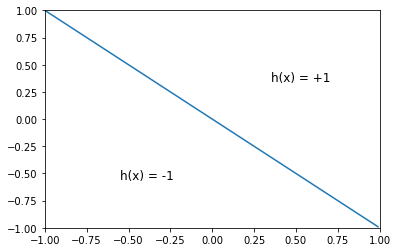
\includegraphics{2.15/1}
    \item Based on the hint, if we have a set of points generated by first choosing one point \math{\mathbf{x_1}} and generating the next one by increasing \math{x_{11}} and decreasing \math{x_{12}}, the new points can either be classified as +1 or -1 no matter the result of \math{\mathbf{x_1}}. In this case, \math{m(H) = 2^N}. Thus, based on the definition, \math{d_{vc} = \infty}
\end{enumerate}

\section{Problem 2.24}

\begin{enumerate}[a)]
    \item For any data set \math{D = \{(x_1, {x_1}^2), (x_2, {x_2}^2)\}}, we have our g can be solved as:
         \begin{equation}
                \begin{cases}
                    x_1a + b = {x_1}^2 \\
                    x_2a + b = {x_2}^2 \\
                \end{cases}   
            \end{equation}
    So we will have 
         \begin{equation}
                \begin{cases}
                    a = x_1 + x_2 \\
                    b = -x_1x_2 \\
                \end{cases}   
            \end{equation}
    We may put the result into our equation below: 
        \begin{equation}
            \begin{split}
                \bar{g}(x) &= E_D[g^D(x)] \\
                &= E_x[ax+b] \\
                &= xE_x[a] + E_x[b] \\
                &= xE_x[x_1 + x_2] + E_x[-x_1x_2] \\
                &= xE_x[x_1] + xE_x[x_2] - E_x[x_1]E_x[x_2]
            \end{split}
        \end{equation}
        Since x is uniformly distributed over \math{[-1, 1]}, we will have \math{E_x[x] = \frac{1}{2}\int^{+1}_{-1}xdx = 0}. Continue we have:
         \begin{equation}
            \begin{split}
                \bar{g}(x) &= xE_x[x_1] + xE_x[x_2] - E_x[x_1]E_x[x_2] \\
                &= x * 0 + x * 0 - 0 * 0 \\
                &= 0
            \end{split}
        \end{equation}
    \item Repeatably generate D with two random points where each components within \math{[-1, 1]}. For each iteration, we compute the linear function \math{g^{D} = (x_1 + x_2)x - x_1x_2}. We will run N iterations, and then generate N points (noted as \math{(y_j, y_j^2)}) randomly for \math{E_{out}}. 
    \begin{itemize}
        \item [\math{\bar{g}}] \math{\frac{1}{N}\sum_{n=1}^N g_n(x)}
        \item [\math{E_{out}}] \math{\frac{1}{N^2} \sum_{i=1}^N \sum_{j=1}^N (g_i(y_j) - f(y_j))^2}
        \item [bias] \math{\frac{1}{N}\sum_{n=1}^N \frac{1}{2} (\bar{g}(x_n) - f(x_n))^2 = \frac{1}{2N}\sum_{n=1}^N ((\bar{g}(x_{n1}) - f(x_{n1}))^2 + (\bar{g}(x_{n2}) - f(x_{n2}))^2) }
        \item [var] \math{\frac{1}{N^2} \sum_{i=1}^N \sum_{j=1}^N (g_i(x_{j}) - f(x_{j}))^2 = \frac{1}{N^2} \sum_{i=1}^N \sum_{j=1}^N ( (g_i(x_{j1}) - f(x_{j1}))^2 + (g_i(x_{j2}) - f(x_{j2}))^2)} 
    \end{itemize}
    \item We set \math{N = 1000} and run the experiment
        \begin{itemize}
            \item [\math{\bar{g}}] \math{-0.0040262929933741615x + 0.0004861293089235126}
            \item [\math{E_{out}}] 0.5312093090854838
            \item [var + bias] 0.528981041701871
            \item [var] 0.33298871628951815
            \item [bias] 0.1959923254123528
        \end{itemize}
        It is observed that \math{E_{out} \approx var + bias} \\
        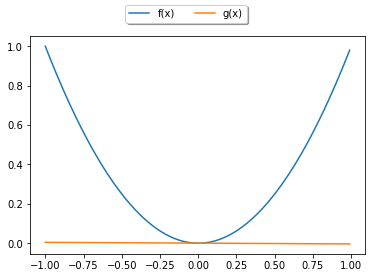
\includegraphics{2.15/2}
    \item 
        \begin{itemize}
            \item [bias]
                \begin{equation}
                    \begin{split}
                        (\bar{g}(x) - f(x))^2 &= \frac{1}{2} \int^1_{-1} (x^2)^2dx \\
                        &= \frac{1}{5}
                    \end{split}
                \end{equation}
            \item [var] 
                \begin{equation}
                    \begin{split}
                        E_x[E_{D}[{(g^D(x) - \bar{g}(x))}^2]] &= \frac{1}{2}\int^1_{-1}\frac{1}{2}\int^1_{-1}\frac{1}{2}\int^1_{-1}((x_1 + x_2)x - x_1x_2)^2 dx_1dx_2dx \\
                        &= \frac{1}{8}\int^1_{-1}\int^1_{-1}\int^1_{-1} (x_1^2 + 2x_1x_2 + x_2^2)x^2 - 2x(x_1^2x_2+x_1x_2^2) + (x_1x_2)^2 dx_1dx_2dx \\
                        &= \frac{1}{8}\int^1_{-1}\int^1_{-1} (\frac{2}{3} + x_2^2)x^2 - \frac{4}{3}x_2 + \frac{2}{3}x_2^2 dx_2dx \\
                        &= \frac{1}{8} \int^1_{-1} \frac{4}{3}x^2 + \frac{4}{9} dx \\
                        &= \frac{1}{8}(\frac{16}{9} + \frac{8}{9}) \\
                        &= \frac{1}{3}
                    \end{split}
                \end{equation}
            \item [\math{E_{out}}] 
                \begin{equation}
                    \begin{split}
                        bias + var &= \frac{1}{5} + \frac{1}{3} \\
                        &= \frac{8}{15}
                    \end{split}
                \end{equation}
        \end{itemize}
\end{enumerate}

\end{document}
